% !TeX root = ../Thesis.tex

%*****************************************
\chapter{Related Work}\label{ch:relatedwork}
%*****************************************
\glsresetall % Resets all acronyms to not used

As \cref{ch:background} has manifested, the desire for privacy is something fundamental to humans, and they have been highly inventive in how to implement mechanisms that preserve it. The modern fruits of this labour are the fields of cryptography and steganography. While cryptography is strict, requiring rigorous mathematics and peer reviews, steganography allows us to be more creative - some even call it an "ancient art"~\cite{bennettLinguisticSteganographySurvey2004}. This is enabled by violating Kerckhoffs' principle: Kerckhoffs demands that a \textit{cryptographic} system should remain secure even if an attacker knows everything about the system, except the secret key~\cite{andersonLimitsSteganography1998}. This can be rephrased as not to rely on security through obscurity, or as Claude Shannon said it: "assume that the enemy knows the system"~\cite{shannonCommunicationTheorySecrecy1949}. In steganography, we don't necessarily deal with secret keys. But the security of our \textit{steganographic} system partially relies on the attacker not knowing which of the countless possibilities we chose to hide data in other data - and that we did it in the first place.

Therefore, an exhaustive discussion of text-based steganography methods related to the implementation presented in this thesis is not possible. Instead, this chapter will go through some selected works, in chronological order. The selection is limited to text-based steganography methods that are suitable for digital communication, as there are text-based methods that might be more suitable for printed text (e.g. encoding information by shifting words or lines~\cite{lowDocumentMarkingIdentification1995}). We progress from simple to more sophisticated approaches, highlighting their advantages and disadvantages over our implementation. This allows us to answer the question: Why use \glspl{LLM} at all?

\section{Text-based steganography without \glspl{LLM}}
\label{sec:textBasedSteganographyWithoutLLMs}
Text-based steganography methods can be grouped into two categories: edit-based or generation-based~\cite{zieglerNeuralLinguisticSteganography2019,bennettLinguisticSteganographySurvey2004}. In edit-based approaches, the cover text is a user input that gets edited to encode information~\cite{zieglerNeuralLinguisticSteganography2019}. In generation-based approaches, the cover text is generated token-wise, with information is being encoded through the selection of each token~\cite{zieglerNeuralLinguisticSteganography2019}. As the rapid progress made in \glspl{LLM} since the introduction of the Transformer architecture~\cite{vaswaniAttentionAllYou2023} is still very young, historcal steganography approaches had to deal with the very limited ability of generating semantically meaningful text. This made edit-based approaches attractive, even though their encoding efficiency is an order of magnitude lower~\cite{zieglerNeuralLinguisticSteganography2019}.

\subsection{Whitespaces}
\label{sec:whitespaces}
A demonstration of edit-based steganography from as early as the year 2000 is still available online today at Spammimic~\cite{spammimicSpammimic2000,dembartEndUserHide2001,bennettLinguisticSteganographySurvey2004}. It takes both a secret message and a cover text as user inputs, then edits the cover text by inserting whitespaces to encode the secret message. \cref{fig:spammimicWhitespaces} shows an example output.

\begin{figure}
    \begin{wide}
        \centering
        \captionsetup{width=\linewidth}
        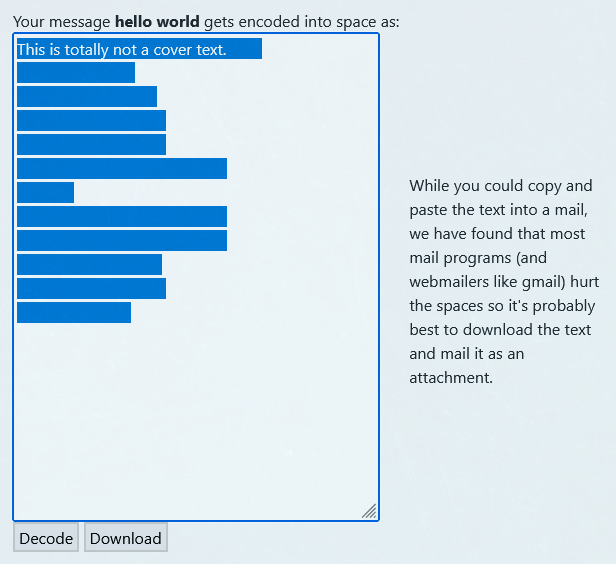
\includegraphics[width=0.75\linewidth]{spammimic_whitespaces.png}
        \caption[Spammimic: Whitespaces]{Steganography in whitespaces with Spammimic~\cite{spammimicSpammimic2000}, made visible by highlighting the text. Both the secret message "hello world" and the unedited cover text "This is totally not a cover text." were user inputs.}
        \label{fig:spammimicWhitespaces}
    \end{wide}
\end{figure}

The strength of this approach in particular is that it is very unlikely to be spotted by an attacker. Unnecessary whitespaces are created regularly by any user of a computer, e.g. as a result of formatting errors or as leftovers from editing a text. As only whitespaces are added, the user has full control over cover text quality. Furthermore, this approach can be transferred to text that is not natural language, i.e. to programming languages. Most programming languages do not rely on whitespaces for their semantics, but use explicit syntax like braces, brackets and parentheses. Encoding a secret message into whitespaces of code would therefore be very likely to keep the program functional. Assuming changes are tracked via a version control system such as Git, the integrity of the cover text would also be ensured.

But the whitespace approach is prone to fail in many typical scenarios of everyday life, where natural language is relevant. Furthermore, it loses an important advantage of text-based steganography over other steganography areas such as image-based steganography, which is independence from the communication medium. Cover texts can not only be sent digitally, but can also be hand-written in a letter or printed in a newspaper, or said over a phone call. If any of the latter is done with an edited cover text as shown in~\cref{fig:spammimicWhitespaces}, it will get corrupted. Whitespaces are lost in non-digital communication channels, rendering the encoded secret message unrecoverable. But this is even possible when using digital communication channels, as~\cref{fig:spammimicWhitespaces} mentions too. Many e-mail clients and instant messengers trim leading and trailing whitespaces to save on bandwidth~\cite{shirali-shahrezaTextSteganographySMS2007}, which would again corrupt the cover text.

\subsection{Mimicking}
\label{sec:mimicking}
Spammimic offers generation-based approaches without involving \glspl{LLM}~\cite{spammimicSpammimic2000}. Most notably, secret messages can be encoded into spam e-mails (hence the name). \cref{fig:spammimicSpamEmail} shows an example output. This is done using context-free grammars and mimic functions (which are the inverse of the Huffman compression function we will use later)~\cite{waynerMimicFunctions1992,bennettLinguisticSteganographySurvey2004}.

\begin{figure}
    \begin{wide}
        \centering
        \captionsetup{width=\linewidth}
        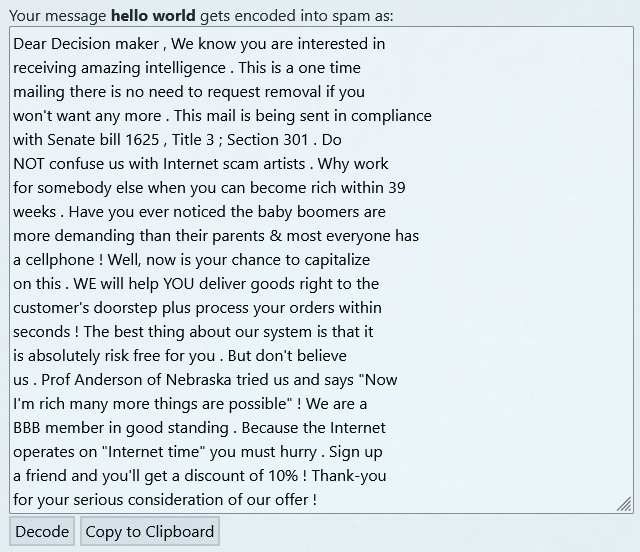
\includegraphics[width=0.75\linewidth]{spammimic_spam_email.png}
        \caption[Spammimic: Spam e-mail]{Steganography in spam e-mails with Spammimic~\cite{spammimicSpammimic2000}. Only the secret message "hello world" was user input.}
        \label{fig:spammimicSpamEmail}
    \end{wide}
\end{figure}

This approach already introduces a number of benefits. Plausible cover texts for a given topic are generated with minimal computing resources, as the output is returned seemingly instantaneous. The choice of spam e-mails as a topic is particularly beneficial, as it will lower an attacker's expectation of cover text quality considerably. Consequently, reading spam e-mails is rather tiring, so an attacker would have to resort to a statistical steganalysis to find irregularities. As spam e-mails are a common part of modern everyday life, cover texts could even be "broadcast" to any number of recipients that includes the intended one. This would obfuscate who is communicating with whom, thereby causing the attacker high costs in searching for the secret message~\cite{bennettLinguisticSteganographySurvey2004,petitcolasInformationHidingSurvey1999}. The vast majority of unintended recipients is likely to delete it without a second thought and would therefore not pose a security risk. Arbitrary plain text messages (i.e. spam e-mails that don't encode a secret message) could be sent in-between to make steganalysis harder by obfuscating when secret communication is happening. Lastly, this approach is robust when using non-digital communication channels, as it does not rely on whitespaces.

But there are still several signifcant drawbacks to the spam e-mail approach. As can quickly be seen when playing around with Spammimic, the cover texts it generates are repetitive. This makes a statistical steganalysis seem promising, e.g. trying to map the letters of the alphabet in the secret message to certain phrases in the generated cover text. The topic of cover texts is hard to exchange as a corresponding grammar is needed, whose creation or acquisition in turn requires expert knowledge. This is not comparable to \glspl{LLM}, where behaviour is controlled via a system prompt that can be exposed to any layman user as a natural language text input. Lastly, encoding is very inefficient here. Any secret message longer than a few words creates cover texts of implausible length, even for a spam e-mail.

\subsection{Substitution}
\label{sec:substitution}
While the last approach was able to generate general purpose cover texts, it is not suitable to create a chat conversation between them - which is a central requirement for our implementation. To combat this, we take a step back and consider an edit-based approach again, as shown in~\cite{shirali-shahrezaTextSteganographySMS2007}. When \gls{SMS} was the prevalent form of mobile communication, it came with a character limit to save on bandwidth. This led to users abbreviating common terms in their conversations, developing their own terminology~\cite{shirali-shahrezaTextSteganographySMS2007} (e.g. "u" instead of "you"). While character limits are not an issue anymore with modern instant messengers, abbreviations persisted as part of internet culture.

We can leverage this to encode information in chat messages. First, we define a dictionary of common terms and their abbreviations. Then, we let the user write their chat message that serves as the unedited cover text. We edit the cover text by searching for terms that appear in our dictionary, then either replacing them with their abbreviation or leaving them in their full form (and vice versa). Any occurence of a term from our dictionary in full form is interpreted as a 0 bit, while usage of an abbreviation is interpreted as a 1 bit~\cite{shirali-shahrezaTextSteganographySMS2007}.

The major advantage of this approach is that a semantically meaningful conversation is ensured by letting users input the unedited cover texts (similar to the whitespace approach described above). As terms and their abbreviations are synonymous, no substitution can change any of the semantics. It is rather accessible for the user as individualizing the dictionary would only require a simple \gls{UI} and no expert knowledge, benefitting cover text quality further. This already covers a lot of the requirements for our implementation - so again, why should we use a \gls{LLM}?

This substitution approach still comes with signifcant downsides. Even with a large dictionary, lots of terms just don't have an abbreviation in practice. Consequently, efficiency is rendered low when a signifcant proportion of terms in the edited cover text doesn't encode any information. This is aggragavated when using abbreviations for entire phrases (e.g. "ily" instead of "i love you"), as it requires the conversation to have more content than when only using abbreviations for individual words. Use of abbreviations can be undesired to improve the readability of messages. Transferring this approach to other, more formal types of conversations can even be inappropriate (e.g. a business e-mail instead of a private chat). Other substitution approaches, i.e. substituing more general synonyms instead of abbreviations specifically, solve these problems only partially. Unlike \glspl{LLM}, these approaches don't consider the context the word being substituted is in. This makes it harder to maintain a semantically meaningful text after the substitution.

\subsection{Further considerations}
\label{sec:furtherConsiderations}
In the previous sections of this chapter, we discussed several approaches for text-based steganography without \glspl{LLM}. In particular, we focussed on the extent to which each approach fulfilled our central requirement - creating a believable chat conversation from cover texts. In this section, we take a look at some more text-based steganography approaches, still without involving \glspl{LLM}. But the focus is now on some more refined requirements, stemming from more specific use cases. Lastly, we take a look at an example of what not to do.

\subsubsection{Localization}
\label{sec:localization}
The overall goal of our implementation can be stated as follows: Use text-based steganography in chat messages to protect against attackers. While multiple aspects of this definition can and will be refined over the course of this thesis, we now want to discuss one aspect that is largely omitted otherwise: Localization. Our standard assumption is that both users and attackers are English-speaking. This may be fine for academic purposes, but in practice a lot of the potential users of our implementation are in countries where English is not an official language. This is especially relevant for protection from political persecution under authoritarian regimes.

An example implementation of location-specific steganography is Nahoft~\cite{united4iranNahoft2021,united4iranU4iadminNahoft2025}. This is an Android app designed to protect people in Iran protesting against their government. It performs text-based steganography by creating cover texts consisting of random Persian words, the official language of Iran. If English was used in this situation, it would only attract unwanted attention from the authorities.

Characteristics specific to languages with non-Latin scripts can be leveraged for steganography. Examples for such languages are Arabic~\cite{shirali-shahrezaNewApproachPersian2006,hamzahLinguisticSteganographyFramework2021,thabitComparativeAnalysisArabic2021}, Chinese~\cite{luoTextSteganographyHigh2017} and Hindi~\cite{allaEvolutionHindiText2009}. The scripts of these languages provide a rich variety of symbols and variations, exceeding what the Latin script has to offer, allowing e.g. multiple equivalent shapes for the same expression~\cite{shirali-shahrezaNewApproachPersian2006,hamzahLinguisticSteganographyFramework2021,thabitComparativeAnalysisArabic2021}. Furthermore, relationships between languages should be considered. Steganography approaches leveraging language-specific characteristics can sometimes be transferred to related languages~\cite{allaEvolutionHindiText2009}.

The challenge of localization can partially be solved with our implementation. As~\cref{ch:design} will explain in detail, one goal of our implementation is that the \gls{LLM} can be swapped out easily. While this doesn't enable us to leverage language specifics like changing character shapes, it enables us to choose a \gls{LLM} that was trained on any natural language desired. If we are able to generate semantically meaningful cover texts in any language, further localization might not be necessary. We could use our implementation in any geo-political conflict, deliberately speaking (or not speaking) the language of the attacker. But verifying this is unfortunately out of scope for this thesis, as the author doesn't speak any languages with non-Latin scripts.

\subsubsection{A negative example}
\label{sec:aNegativeExample}
Lastly, we want to take a look at an example of what not to do, so we can avoid it in our implementation. We recall that steganography violates Kerckhoffs' principle~\cite{andersonLimitsSteganography1998}, as the security of a steganographic system partially relies on the attacker not knowing the system - or that it is being used in the first place.

An approach for text-based steganography in e-mails is shown in~\cite{malikHighCapacityText2017}. Similar to our implementation, it uses Huffman compression to convert a secret message from string to binary. But instead of generating a cover text with \glspl{LLM}, an edit-based approach is chosen by taking the cover text from user input. Information is encoded by colour coding the cover text, with colours being selected from a user-defined colour table. \cref{fig:colourCoding} shows the example given in~\cite{malikHighCapacityText2017}. As~\cite{malikHighCapacityText2017} proposes, this approach is suitable for personal messages containing congratulations, poems, etc. Users may try to obfuscate the steganography as they have full control over cover text quality and the colour table, e.g. by choosing black, dark grey, light grey and white as colours.

\begin{figure}
    \begin{wide}
        \centering
        \captionsetup{width=\linewidth}
        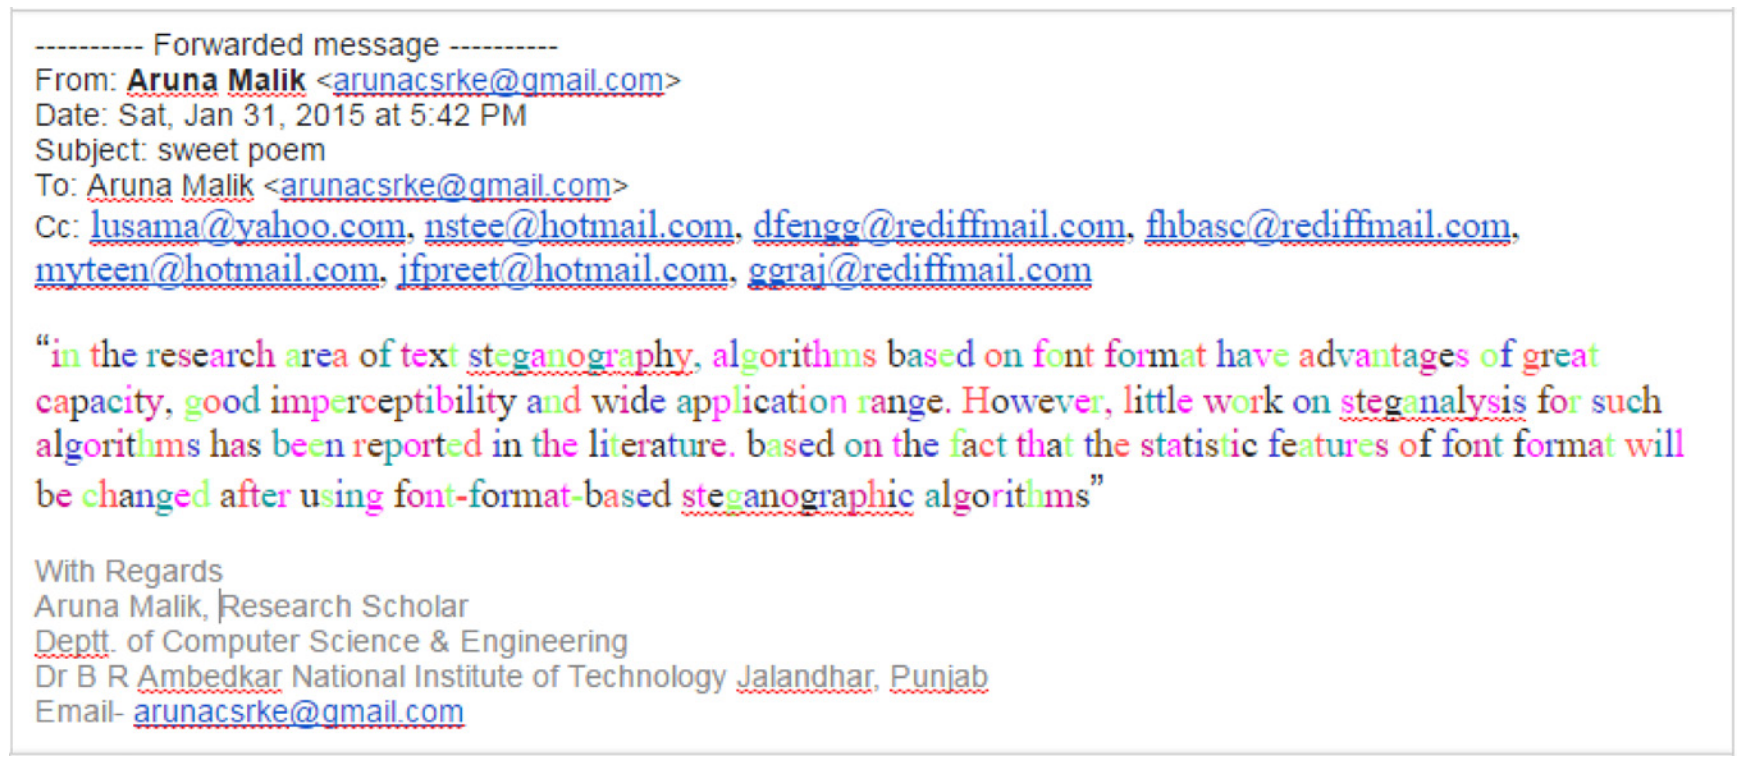
\includegraphics[width=0.75\linewidth]{colour_coding.png}
        \caption[Colour coding]{Steganography via colour coding~\cite{malikHighCapacityText2017}.}
        \label{fig:colourCoding}
    \end{wide}
\end{figure}

However, this doesn't outweigh the disadvantages. The colour table has to be exchanged between sender and receiver, which is difficult as it is not natural language. This approach also is not robust when using non-digital communication channels, as the colour coding is lost if the cover text is spoken during a phone call or printed out in black and white. The proposed use case is very narrow, as an attacker should become suspicious if this is used in any other setting. More generally, the colour coding introduces an unnatural communication pattern that might make it obvious to an attacker that a secret communication is happening. This breaks the additional layer of security that is supposed to be introduced by steganography. We can transfer this to our implementation by avoiding e.g. uncommon use of abbreviations or emojis in the generated chat conversations. Furthermore, we should also avoid introducing unnatural restrictions, e.g. assuming that chat messages are being sent with strictly alternating roles of sender and receiver. \cref{ch:implementation} will show that this is only partially possible in our implementation.

\section{Text-based steganography with \glspl{LLM}}
\label{sec:textBasedSteganographyWithLLMs}
In the last section, we investigated how text-based steganography can be performed without involving \glspl{LLM}. Historical approaches were mostly edit-based, as the ability to generate coherent text was limited~\cite{zieglerNeuralLinguisticSteganography2019}. This changed with the introduction of the Transformer architecture~\cite{vaswaniAttentionAllYou2023} in 2017, which laid the foundation for the popular \gls{AI} chatbots we know today.

In this section, we first consider high-level approaches that only involve prompting the \gls{LLM} to perform steganography. Then, we consider low-level approaches that manipulate the token generation of the \gls{LLM}. This finally leads us to the paper this thesis is based on~\cite{zieglerNeuralLinguisticSteganography2019}.

\subsection{High-level: Prompting}
\label{sec:highLevelPrompting}
With state-of-the-art \glspl{LLM} reaching hundreds of billions of parameters, they are able to comprehend long contexts and perform advanced logic only by being prompted~\cite{hossainLLMProSAnalyzingLarge2025}. \gls{AI} chatbots like ChatGPT help users solve problems in all fields of science and engineering~\cite{schmidgallAgentLaboratoryUsing2025}, from solving physics equations~\cite{songLLMFeynmanLeveragingLarge2025,panQuantumManybodyPhysics2025} to writing and debugging code~\cite{leeGitHubRecentBugs2024,leeUnifiedDebuggingApproach2024,tianDebugBenchEvaluatingDebugging2024,shiCodeCorrectnessClosing2024}. This suggests that we might be able to instruct a \gls{LLM} to behave like a steganographic system, i.e. to generate a cover text that encodes a secret message.

As demonstrated in~\cite{steinebachNaturalLanguageSteganography2024,wuPromptingSteganographyNew2024} with ChatGPT, it is possible to perform steganography by prompting \glspl{LLM}. We will focus on~\cite{steinebachNaturalLanguageSteganography2024}, as its approach is simpler and the relevant advantages and disadvantages are similar to~\cite{wuPromptingSteganographyNew2024}.

A possible approach to perform steganography via prompting works as follows (simplified)~\cite{steinebachNaturalLanguageSteganography2024}: Define two disjoint sets of words, A and B. Instruct the LLM to generate a text that contains words from A and B matching a certain pattern (e.g. BABBABABA). Interpret any occurence of a word from set A as a 0 bit, any of a word from set B as a 1 bit. Use this logic to define a pattern matching the desired bit sequence, thereby encoding a secret message in the generated cover text.

This approach is attractive because it only requires high-level access to the \gls{LLM}. The user doesn't need to understand technical details like tokenization or tensors to influence the behaviour of the \gls{LLM}. The topic of the cover text can be controlled via the words in sets A and B, which themselves can be generated with a single prompt. Efficiency can be improved by increasing the number of sets to choose from~\cite{steinebachNaturalLanguageSteganography2024}, thereby encoding more bits of information within every selected word. It is also relatively efficient in computing resources, as the \gls{LLM} is only needed for encoding, while decoding can be performed deterministically given a cover text and the word sets. Quality of cover texts can too be controlled easily. If a previously generated cover text is not satisfactory, only reprompting is needed. This suggests that generating a conversation from cover texts is plausible too.

Although this approach may be able to fulfill the central requirement for our implementation, it conflicts with almost every other goal and requirement we set ourselves. As even the largest \glspl{LLM} struggle with reliability~\cite{vendrowLargeLanguageModel2025}, they still make encoding errors with the careful prompt engineering demonstrated in~\cite{steinebachNaturalLanguageSteganography2024,wuPromptingSteganographyNew2024}, thereby corrupting the secret message. For any smaller \gls{LLM} that is feasible to run locally on a smartphone, this will be aggragavated. This would make the core functionality of our implementation dependent on cloud-based, largely closed source service providers. These providers have commercial interest in our personal data and would be able to tie the secret messages to our identities. Furthermore, for many users these service providers would not be in their jurisdiction. Foreign law enforcement could therefore demand and obtain access to user data without users being aware of it or having any legal recourse. This approach is not to be desired as availability would not be ensured. While large commercial service providers generally have good uptime records, an implementation relying on them would require a constant internet connection and access to the provider's domain. Recalling the use case of protection from authoritarian regimes mentioned in~\cref{sec:localization}, the latter is a non-trivial assumption, as such regimes often block undesirable domains country-wide~\cite{wongSocialMediaMay2016,michaelsonJournalistsMore11002025}. Lastly, even though this is a generation-based approach, encoding efficiency is not very high. While it can be controlled via the number of word sets as described above, the examples given in~\cite{steinebachNaturalLanguageSteganography2024} show that most words in the cover text don't encode any information. This suggests that the simplicity of this approach is not worth largely giving up privacy and immensely increasing the attack surface.

\subsection{Low-level: Manipulating token generation}
\label{sec:lowLevelManipulatingTokenGeneration}
The last section reinforced several further requirements for our implementation: It should be local-first and work offline to introduce as little third party dependencies as possible. We cannot rely on commercial providers for access to the most powerful \glspl{LLM}, but have to run a smaller \gls{LLM} locally. This restricts the possible complexity of prompts significantly (see~\cref{ch:design} for details), leading us to consider a more low-level approach to influence the behaviour of the \gls{LLM}.

A possible approach is demonstrated in Stegasuras~\cite{zieglerNeuralLinguisticSteganography2019,zieglerHarvardnlpNeuralSteganography2025,zieglerStegasuras2025}, which serves as the foundation for this thesis. It implements steganography by manipulating the token generation of the \gls{LLM}. This requires low-level access to tokenizers and tensors, which none of the previous approaches considered. Arithmetic, Huffman and Bins encoding algorithms are implemented using GPT-2 and PyTorch (see~\cref{ch:design} and~\cref{ch:implementation} for corresponding details of our implementation).

This approach is promising several strengths we haven't seen before. By gaining low-level access to the \gls{LLM}, we can implement a complex encoding logic. This wouldn't be possible via prompting due to the limited selection of \glspl{LLM} imposed by the restrictions of mobile devices. It allows us to reach a significantly higher encoding efficiency than previous approaches~\cite{zieglerNeuralLinguisticSteganography2019}.

Fundamentally, it works as follows: A secret message is first converted from string to binary. A cover text is then generated by selecting tokens from the predictions of the \gls{LLM} for a given context. This selection is based on a logic that processes the secret message bits, thereby encoding information within each selected token~\cite{zieglerNeuralLinguisticSteganography2019}. The logic by which the tokens are selected can be exchanged, i.e. the three algorithms mentioned above can be seen as one generic algorithm with a variable sampling method.

Arithmetic coding is used not only for steganography, but also for compressing the secret message during its binary conversion~\cite{zieglerNeuralLinguisticSteganography2019}. For long strings with known probability distribution this compression is optimal, i.e. it compresses them to their entropy~\cite{rissanenArithmeticCoding1979}. In practice, it is often more efficient than Huffman compression~\cite{zieglerNeuralLinguisticSteganography2019} (see~\cref{ch:implementation} for further discussion). This further increases encoding efficiency and lowers the barrier for small \glspl{LLM} to generate believable cover texts.

While this suggests that steganography with local \glspl{LLM} might be feasible on smartphones, the implementation demonstrated in~\cite{zieglerStegasuras2025} is not without issues. Most notably, being published in 2019, it is not state-of-the-art anymore. Significant gains in cover text quality are to be expected by just swapping out the \gls{LLM}.

Furthermore, there is an edge case that is not covered in any of the implemented algorithms. While encoding, the \gls{LLM} will generate cover text tokens until all bits of the secret message are processed. As it stands, this would mean that token generation ends abruptly while the cover text might be in the middle of a sentence. Such a cover text would look highly suspicious to an attacker, rendering this approach unusable for creating believable chat conversations. While the code provided at~\cite{zieglerHarvardnlpNeuralSteganography2025} already contains a flag to finish the last sentence of the cover text by greedy sampling, it is not used. Simply setting this flag from \lstinline|false| to \lstinline|true| doesn't solve the issue though, since the decoding functions don't consider it. This creates noise when recovering a secret message, as tokens from greedy sampling don't contain any information.

While this issue is important to factor in when judging cover text quality and therefore real world use, it is ignored in the evaluation of Stegasuras~\cite{zieglerNeuralLinguisticSteganography2019}: Participants were presented four sentences of text, the first three taken from news articles and used as context, the last one generated by the \gls{LLM}. They were then asked to judge if the fourth sentence is a plausible continuation of the first three. Any output of the \gls{LLM} longer than one sentence was cut off~\cite{zieglerNeuralLinguisticSteganography2019}, thereby corrupting the cover text and rendering the secret message unrecoverable. A more sensible solution would have been to let the \gls{LLM} finish its last sentence and to clean up the noise in decoding.

Improving the implementation by solving this challenge is the first contribution this thesis makes (see \cref{ch:implementation} for our solution). Beyond that, the value of this thesis is created in multiple ways. The implementation will be extended to generate a believable chat conversation from cover texts. This is done by leveraging the context that is passed to the \gls{LLM} (see \cref{ch:implementation}). We will show that it is feasible to run all of this locally on a smartphone by the example of the Android platform. We provide our own implementation using a state-of-the-art framework (see \cref{ch:design}). We will show how to handle irregularities in human communication (e.g. sending plain texts in-between cover texts, using emojis or allowing multiple consecutive messages from the same sender). Lastly, we will increase control over cover text quality further by not just passing a context to the \gls{LLM}, but also by implementing a system prompt for easy low-level access. This way, we are able to solve the real-world use case of protecting people from attackers with steganography.
